\documentclass[../main.tex]{subfiles}
\begin{document}
\section{Introduction}
\label{sec:intro}
\begin{figure}[h]
    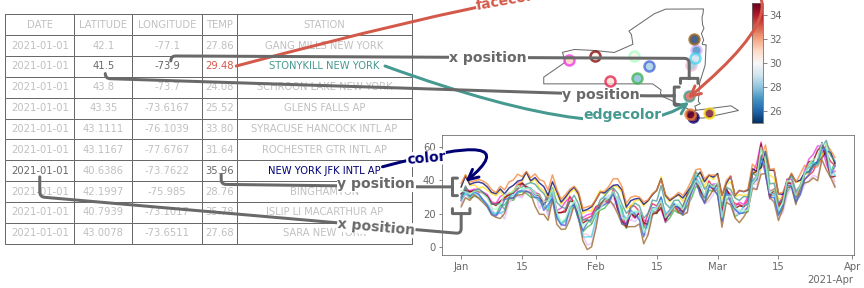
\includegraphics[width=1\textwidth]{figures/intro/functions.png}
    \caption{Building block visualization libraries implement independent reusable functions that map data to visual representations. For example, position encoding functions map the latitude and longitude values in the table (a) to locations on the map (b). These same encoding functions map dates and precipitation (a) to x and y positions in the timeseries plot (c). Color encoding functions map the precipitation (a) to the color of the point in the map (a) and color encoding functions map names of weather stations (a) to colors in both the map (a) and timeseries (b). Functions, which we call \textit{artists}, compose these encoding functions into attributes of visual elements. The \texttt{point} artist transforms the output of the position, facecolor, and edgecolor maps into attributes of each point in the map (a), while the \texttt{line} artist transforms the output of the position and color maps into attributes of each line in the timeseries plot (c).}
    \label{fig:intro:artist}
\end{figure}

Visualizations, by definition, reflect something of the underlying structure and semantics\cite{friendlyBriefHistoryData2008} of the data, whether through direct mappings from data into visual elements or via figurative representations that have meaning due to their similarity in shape to external concepts \cite{byrneAcquiredCodesMeaning2016}. We define visualization components to be structure preserving maps from data to visual representations. As illustrated in \autoref{fig:intro:artist}, visualizations map weather station precipitation data (a) into graphical elements such as points (b) and lines (c) and map individual data components (columns) into components of the visualization such as position or color. For example, the gray position encoder function converts the latitude and longitude to x and y positions, and the color encoders map temperature and station name to colors. A \texttt{point} function composites these encodings into attributes of a point in the map (a). The \texttt{line} function composites encoders that convert station name to color and date and precipitation to x and y positions into a piece of a line in the timeseries plot (c). We identify the structure these maps must preserve as the \textit{continuity} of the data and the \textit{equivariance} of the data and visual components. 

We introduce a model of visualization components based on these \textit{continuity} and \textit{equivariance} constraints and use this model to develop a design specification. Our specification is targeted at building block libraries, as defined by Wongsuphasawat\cite{wongsuphasawatNavigatingWideWorld2021}, because they are the visualization tools that provide independent functions that map components of data to visual representations.  Just as the number of ways to arrange physical building blocks is solely constrained by the size and shape of the blocks, we propose that the only restriction on how building block library components can be composed are that the compositions preserve \textit{continuity} and \textit{equivariance}. Independent, modular, components are inherently functional\cite{hughesWhyFunctionalProgramming1989}, so we propose a functional architecture for our model. Doing so means the functional architecture can be evaluated for correctness, the resulting code is likely to be shorter and clearer, and the architecture is well suited to distributed, concurrent, and on demand tasks\cite{huHowFunctionalProgramming2015}.

This work is strongly motivated by the needs of the Matplotlib\cite{hunterMatplotlib2DGraphics2007,hunterArchitectureOpenSource} visualization library. One of the most widely used visualization libraries in Python, new components and features have been added in an organic, sometimes hard to maintain, manner since 2002.  In Matplotlib, every component carries its own implicit notion of how it believes the data is structured-for example if the data is a table, cube, image, or network - that is expressed in the API for that component. This leads to an inconsistent API for interfacing with the data, for example when  updating streaming visualizations or constructing dashboards\cite{a.sarikayaWhatWeTalk2019}. This entangling of data model with visual transform also yields inconsistencies in how visual component transforms, e.g. shape or color, are supported. We propose a redesign of the functions that convert data to graphics, named \textit{Artists} in Matplotlib, in a manner that reliably enforces \textit{continuity} and \textit{equivariance} constraints. We evaluate our functional model by implementing new artists in Matplotlib that are specified via \textit{equivariance} and \textit{continuity} constraints. We then use the common data model introduced by the model to demonstrate how plotting functions can be consolidated in a way that makes clear whether the difference is in expected data structure, visual component encoding, or the resulting graphic.

\section{Background}
There are many formal models of visualization as structure preserving maps from data to visual representation, and many implementations of visualization libraries that preserve this structure in some manner. This work bridges the formalism and implementation in a functional manner with a topological approach at a building blocks library level. We propose a data structure agnostic model of the constraints visual transformations must satisfy such that they can be composed to produce \textit{equivariant} and \textit{continuity preserving} visual representations. 

\subsection{Structure}
\label{sec:intro:structure}
\begin{figure}[H]
        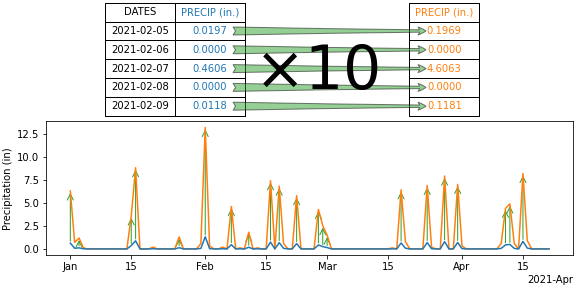
\includegraphics[width=1\textwidth]{figures/intro/equivariant.png}
        \caption{The table (a) lists precipitation in millimeters in blue. These values are converted to  inches, in green, by dividing the millimeter values by 25.4. This conversion is a scaling action, represented by the orange arrows in (a). The \textit{equivariant} action is the scaling in the timeseries (b), which is represented by the orange fill between the green and blue lines. In (c), the scaling is illustrated in the different millimeter and inches y axis labeling of data that appears identical since the distances were scaled by a constant factor that is now incorporated in the labeling.}
      \label{fig:intro:equivariance}
\end{figure}
The components of a visual representation were first codified by Bertin\cite{bertinSemiologyGraphicsDiagrams2011a}, who introduced a notion of structure preservation that we formally describe in terms of \textit{equivariance} and \textit{continuity}. Bertin proposes that there are categories of visual encodings-such as position, shape, color, and texture-that preserve the properties of the measurement type, quantitative or qualitative, of the encoded data. For example, in \autoref{fig:intro:equivariance}, the blue precipitation data in millimeters in the table (a) is converted to inches. This scaling action is represented by the green arrows that translate the precipitation into the scaled values in green. For this visualization to be equivariant, this same scaling factor must be present in the timeseries representation of the data (b). The precipitation in green is an \textit{equivariant} scaling of the precipitation in blue, meaning that the y-values of the green line is $\frac{1}{25.4}$ that of the y-values of the blue precipitation timeseries. The orange fill in the timeseries (b) is the scaling equivalent to the arrows in the table (a). By definition, the distances in the millimeter data were scaled equally \cite{stothersSimilarityGroup} when converted to inches, which means the shapes of the graphs are equivalent when plotted against y-axes that preserve relative distance (c). This visualization is also equivariant to the table (a), but this is indicated through labeling rather than the line plots. The idea of equivariance is formally defined as the mapping of a binary operator from the data domain to the visual domain in Mackinlay's \textit{A Presentation Tool}(APT) model\cite{mackinlayAutomatingDesignGraphical1986, mackinlayAutomaticDesignGraphical1987}. The algebraic model of visualization proposed by Kindlmann and Scheidegger uses equivariance to refer generally to invertible binary transformations\cite{kindlmannAlgebraicProcessVisualization2014}, which are mathematical groups \cite{shadrachIntroductionGroups2017}. Our model defines \textit{equivariance} in terms of monoid actions, which are a more restrictive set than all binary operations and more general than groups. As with the algebraic model, our model also defines structure preservation as commutative mappings from data space to representation space to graphic space, but our model uses topology to explicitly include continuity.

\begin{figure}[H]
    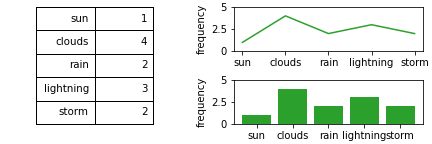
\includegraphics[width=1\textwidth]{figures/intro/continuity.png}
    \caption{The bar chart (b) and line plot (c) are different visual encodings of the precipitation data in the table (a). The bar chart preserves the \textit{continuity} of the stations by encoding the discrete station data as discrete bars (b). In contrast, the line plot (c) does not preserve this discrete \textit{continuity} because it connects the total temperature at each station by drawing a line through each point. Doing so implies that the total temperatures are points along a 1D continuous line, whereas there is no connectivity between the stations or their corresponding rows in the table.}
    \label{fig:intro:continuity}
\end{figure}
The notion that data is equivalent to visual representations when structure is preserved serves as the basis for visualization best practices. When \textit{continuity} is preserved, as in the bar chart (b) in \autoref{fig:intro:continuity}, then the graphic has not introduced new structure into the data.  In \autoref{fig:intro:continuity}, the line plot (c) does not preserve \textit{continuity} because the line connecting the total precipitation of the stations implies that the stations are connected to each other along a 1D continuous line. Bertin asserted that \textit{continuity} was preserved by choosing graphical marks that match the \textit{continuity} of the data - for example discrete data is a point, 1D continuous is the line, and 2D data is the area mark. Informally, Norman's Naturalness Principal\cite{NaturalnessPrincipleInfoVis} states that a visualization is easier to understand when the properties of the visualization match the properties of the data. This principal is made more concrete in Tufte's concept of graphical integrity, which is that a visual representation of quantitative data must be directly proportional to the numerical quantities it represents (Lie Principal), must have the same number of visual dimensions as the data, and should be well labeled and contextualized, and not have any extraneous visual elements\cite{tufteVisualDisplayQuantitative2001}. Expressivity, as defined by Mackinlay, is a measure how much of the mathematical structure in the data can be expressed in the visualizations; for example that ordered variables can be mapped into ordered visual elements. We generalize these different codifications of structure preserving encodings, proposing that a graphic is an equivalent representation of the data when \textit{continuity} and \textit{equivariance} are preserved.

\begin{mdframed}[roundcorner=10pt, frametitle=Structure, frametitlerule=true, frametitlebackgroundcolor=gray!10]
    \begin{description}
        \item[\textbf{continuity}] How elements in the dataset are connected to each other, e.g. discrete points, networked nodes, points on a continuous surface
        \item[\textbf{equivariance}] if an action is applied to the data or the graphic--e.g. a rotation, permutation, translation, or rescaling-- there must be an equivalent action applied on the other side of the transformation. 
    \end{description}
\end{mdframed}



\subsection{Tools}
\label{sec:intro:data:tools}
\begin{figure}[H]
    \begin{subfigure}{.3\textwidth}
        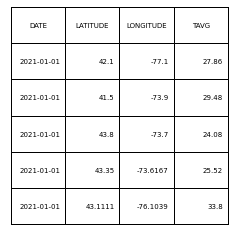
\includegraphics[width=1\textwidth]{figures/intro/table.png}
        \caption{}
        \label{fig:intro:table}
    \end{subfigure}
    \begin{subfigure}{.3\textwidth}
        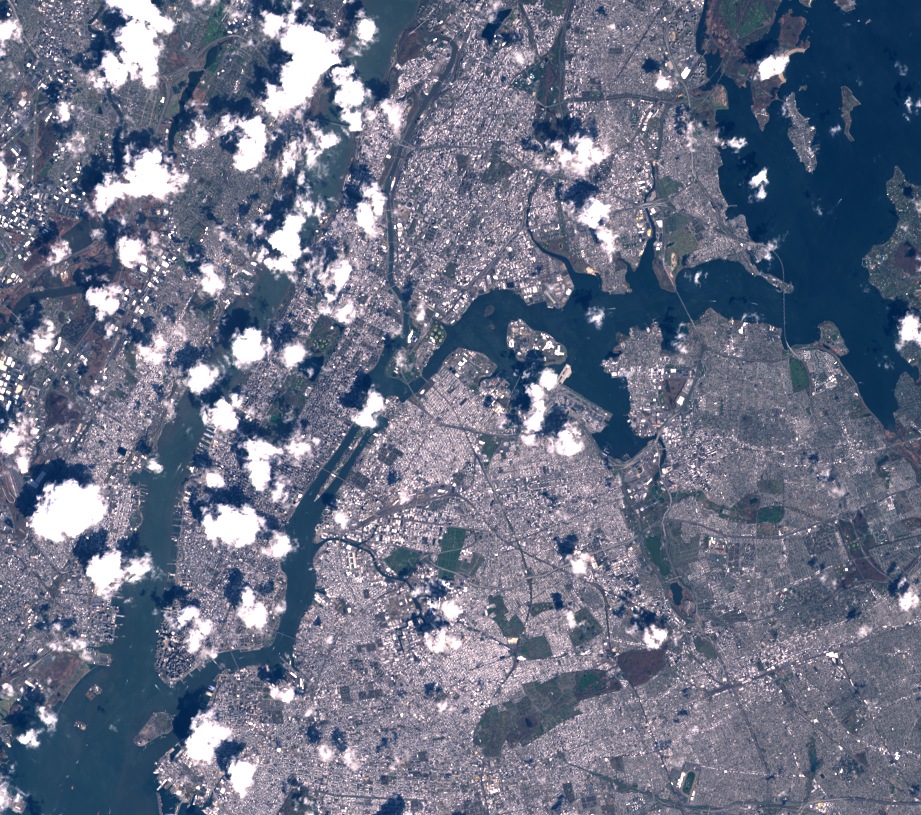
\includegraphics[width=1\textwidth]{figures/intro/landsat.png}
        \caption{}
        \label{fig:intro:image}
    \end{subfigure}
    \begin{subfigure}{.3\textwidth}
        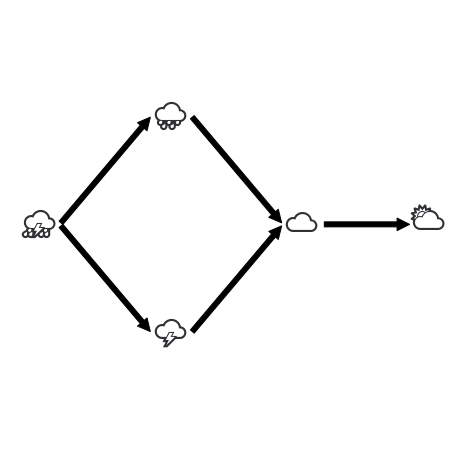
\includegraphics[width=1\textwidth]{figures/math/graph.png}
        \caption{}
        \label{fig:intro:graph}
    \end{subfigure}
    \caption{Visualization libraries, especially ones tied to specific domains, tend to be architectured around a core data structure, such as tables \autoref{fig:intro:table}, images \autoref{fig:intro:image}, or networks \autoref{fig:intro:graph}.
    %%revise as combined fig?
    }
    \label{fig:intro:data}
\end{figure}

Most information visualization software design patterns are tuned to specific data structures and domains, as categorized by Heer and Agrawala\cite{HeerSoftware2006}. For users who generally work in one domain--such relational tables (\autoref{fig:intro:table}), images (\autoref{fig:intro:image}), or graphs (\autoref{fig:intro:graph})--well defined data space (and corresponding visual space\cite{chiTaxonomyVisualizationTechniques2000}) often yields a coherent user experience\cite{heerDeclarative2010}. This coherant experience is often not extensible; developers who want to build new visualizations on top of these libraries must work around the existing assumptions, sometimes in ways that break the architecture model of the libraries. For example tools influenced by APT that assume that data is a relational table integrate computation into the visualization pipeline. This is a wide array of tools, including Tableau\cite{StoltePolaris2002,hanrahanVizQL2006,MackinlayShowme2007} and the Grammar of Graphics\cite{wilkinsonGrammarGraphics2005} inspired ggplot\cite{wickhamGgplot2ElegantGraphics2016a}, protovis\cite{bostockProtoviz2009}, vega\cite{satyanarayanDeclarativeInteractionDesign2014} and altair\cite{vanderplasAltairInteractiveStatistical2018}. Since these libraries represent data as a table, and computations on tables are well defined\cite{ullmanFirstCourseDatabase2008}, these libraries implement computation as part of the visualization process. This is also true of tools that support images, such as the biology oriented ImageJ\cite{schneiderNIHImageImageJ2012} and  Napari\cite{nicholas_sofroniew_2021_4533308} or the digital humanities ImageJ macro ImagePlot\cite{studiesCulturevisImageplot2021}. While these tools often have some support for visualizing non image components of the data, the architecture is oriented towards building plugins into the existing system \cite{WritingPlugins} where the image is the core data structure. Tools like Gephi\cite{bastianGephiOpenSource2009}, Graphviz\cite{ellsonGraphvizOpenSource2002}, and Networkx\cite{HagbergExploringNetwork2008} are used to  visualize and manipulate graphs. As with tables and images, extending network libraries to work with other types of data either requires breaking the libraries internal model of how data is structured and what data transformations are allowed or implementing a model for other types of data structures alongside the network model. Our model aims to identify which computations are manipulations of the data and which are necessary for the visual encoding; for example data is often aggregated for a bar chart but it is not required, while a boxplot by definition requires computing distribution statistics\cite{wickham40YearsBoxplots2011}. Disentangling the computation from the visual transforms allows us to determine whether the visualization library should implement computations or if they should be implemented in data space. 


\begin{figure}[H]
    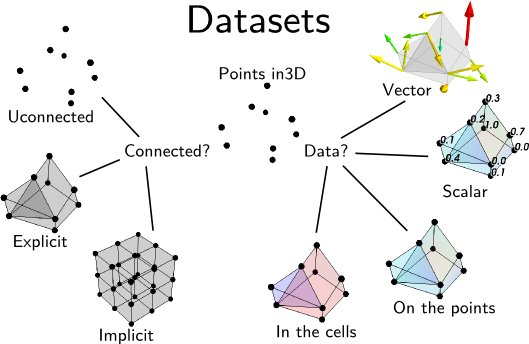
\includegraphics[width=1\textwidth]{figures/intro/dataset_diagram.png}
    \caption{The \textit{continuity} of the data is often used to classify data structures. For example, a relational database often consists of discrete unconnected points, while an image is an implicitly connected 2D grid. This image is from the Data Representation chapter of the MayaVi 4.7.2 documentation.\cite{DataRepresentationMayavi}}
    \label{fig:intro:data:format}
\end{figure}

Visualizations assume the structure of the input data, as described in Tory and Möller's taxonomy \cite{toryRethinkingVisualizationHighlevel2004}, which leads to many building block libraries implementing multiple models of data to support these different visualizations. For example, in Matplotlib, D3\cite{bostockDataDrivenDocuments2011} VTK \cite{hanwellVisualizationToolkitVTK2015,geveciVTK2012} and MayaVi\cite{RamachandranMayaVI2011}, every plot is defined in terms of the \textit{continuity} of the data it expects as input. VTK has explicitly codified this in terms of \textit{continuity} based data representations, as illustrated in figure~\ref{fig:intro:data:format}. Downstream library developers impose some coherency by writing domain specific libraries with assumed data structures on top of the building block libraries--for example Seaborn\cite{waskom2020seaborn} and Titan\cite{brianwylieUnifiedToolkitInformation2009} assume a relational database, xarray\cite{hoyer2017xarray} and ParaView\cite{ahrens2005paraview} assume a data cube--but must work around the incoherencies in the building block libraries to do so. Our model navigates the tradeoff between coherency and extensibility by proposing functional composable well constrained visual components that take as input a structure aware data abstraction general enough to provide a common interface for many different types of data continuities. 


\subsection{Data}
\label{sec:intro:data:continuity}
Fiber bundles were proposed by Butler as a core data structure for visualization because they encode data \textit{continuity} separately from the components of the dataset\cite{butlerVisualizationModelBased1989,butlerVectorBundleClassesForm1992}. Butler's model lacks a robust way of describing variables; therefore we encode a schema like description of the data in the fiber bundle using Spivak's topological description of data types \cite{spivakDatabasesAreCategories2010,spivakSIMPLICIALDATABASES}. In this work, we refer to the points of the dataset as \textit{records}, as defined by Spivak. Each \textit{component} of the record is a single object, such as a precipitation measurement, a station name, or an image. We generalize \textit{component} to mean all objects in the dataset of a given type, such as all precipitation values or station names or images. The way in which these records are connected is the \textit{continuity} or more generally topology.

\begin{figure}[H]
    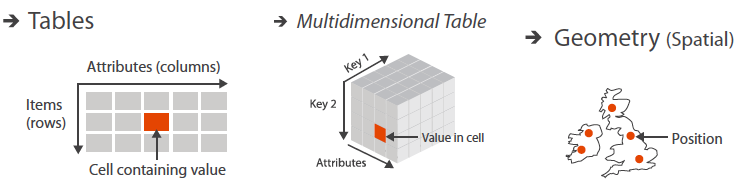
\includegraphics[width=1\textwidth]{figures/intro/munzner_datatypes.png}
    \caption{Values in a dataset have keys associated with them that describe where the value is in the dataset. These keys can be indexers or semantically meaningful;for example, in a table the keys are the variable name and the row ID. In the data cube,  the keys is the row, column, and cell ID, and in the map the key is the position in the grid. Image is figure 2.8 in Munzner's Visualization Analysis and Design\cite{munznerVisualizationAnalysisDesign2014}}
    \label{fig:intro:keys:values}
\end{figure}

The \textit{continuity} can be described in some datasets by components of the dataset. This is formalized by Munzner's notion of metadata as \textit{keys} into the data structure that return associated \textit{values}\cite{munznerChDataAbstraction}. As shown in \autoref{fig:intro:keys:values}, keys can be labeled indexes, such as the attribute name and row ID, or semantically significant physical entities such as locations on a map. In contrast to Munzner's model, in out model components may describe the keys but are never themselves the keys; instead we propose that keys are points on a topological space encoding the continuity of the data. This allows the metadata to be altered without imposing new semantics on the underlying structure, for example by changing the coordinate systems or time resolution. This value agnostic model also supports encoding datasets where there may be multiple independent variables without having to assume any one variable is inducing the change , for example measures of plant growth given variations in water, sunlight, and time. For building block library developers, a non-semantic model of data continuity allows for the implementation of components that can traverse data structures without having to know the semantics of the data. Since these building block components are by design \textit{equivariant} and \textit{continuity preserving}, domain specific library developers in different domains that rely on the same continuity, for example 2D continuity, can use the same components to build tools that can make domain specific assumptions.

\subsection{Contribution}
In this work, we present a framework for understanding visualization as equivariant continuity preserving maps between topological spaces. Using this mathematical formalism, we develop an architecture specification developers can use to implement components in building block visualization libraries that domain specific library developers can carry through in the tools they build. Our work diverges from previous models of visualization and implementations of those models in that it contributes

\begin{enumerate}
  \item formalization of the topology preserving relationship between data and graphic via continuous maps \autoref{sec:math:graphic:base}
  \item formalization of property preservation from data component to visual representation as equivariant maps \autoref{sec:math:artist:nu}
  \item functional oriented visualization architecture built on the mathematical model to demonstrate the utility of the model \autoref{sec:math:artist:q}
  \item prototype of the architecture built on Matplotlib's infrastructure to demonstrate the feasibility of the model. \autoref{sec:code:artists}
\end{enumerate}
We validate our model by using it to re-design artist and data access layer of Matplotlib, a general purpose visualization tool. We evaluate whether the redesign is successful by comparing it to existing implementation, recreating existing domain specific functionality with the new components, and by implementing components that provide new functionality in Matplotlib. While much of this functionality is currently possible in Matplotlib, a functional approach allows us to implement components in a more robust, modular, reliable way.
\end{document}